%%\documentclass[12pt]{article}
\documentclass[12pt]{elsarticle}
\usepackage{graphicx}
\usepackage{subfig}
\usepackage{amssymb,hyperref,rotating}
%\usepackage{draftwatermark}
%\SetWatermarkScale{2.0}
%\usepackage{dcolumn}
%\usepackage{bm}
%\documentstyle{psfig,epsf}{article}
%\usepackage{psfig,wrapfig,floatfig,float}
%\topmargin 0.5cm
%\addtolength{\evensidemargin}{-1.5cm}
%\addtolength{\oddsidemargin}{-1.5cm}
%\addtolength{\textwidth}{2.54cm}
%\addtolength{\topmargin}{-1.5cm}
%\addtolength{\textheight}{2.54cm}

\topmargin=-0.25in
\textwidth=6.25in
\textheight=8.25in
%\textheight=9.25in
\oddsidemargin=0.125in
\evensidemargin=0.125in

%\addtolength{\textwidth}{1.2in}
%\addtolength{\topmargin}{-.7in}
%\addtolength{\leftmargin}{-1.1in}
%\addtolength{\footskip}{-1.5cm}
%%\setlength{\textheight}{9.25in}
%\setlength{\textheight}{9.3in}
%%\setlength{\parindent}{1em}
%\setlength{\parskip}{1ex}
%%\pagestyle{headings}
%\setlength{\oddsidemargin}{0.in}
%\setlength{\evensidemargin}{0.in}
%\renewcommand{\thepage}{Eric D. Church/page \arabic{page}}
\thispagestyle{empty}

\pagestyle{myheadings}
\begin{document}
\title{The Liquid Argon Offline Software Package: LArSoft} 
\author{Jonathan Asaadi}
\address{}
\ead{}
\author{Bruce Baller}
\address{}
\ead{}
\author{Ben Carls}
\address{}
\ead{}

\author{Eric Church}
\address{Yale University, PO Box 500, MS309, Fermi National Accelerator Lab, Batavia, IL, USA, 60510-5011}
\ead{echurch@fnal.gov}
\author{Bonnie Fleming}
\address{Yale University, PO Box XYZ, Physics Department, Yale University, New Haven, CT, USA, 12345-1234}
\ead{bonnie.fleming@yale.edu}
\author{Herb Greenlee}
\address{}
\ead{}
\author{Ben Jones}
\address{}
\ead{}
\author{Wes Ketchum}
\address{}
\ead{}
\author{David McKee}
\address{}
\ead{}

\author{Gianluca Petrillo}
\address{}
\ead{}
\author{Brian Rebel}
\address{PO Box XYZ, MS309, Fermi National Accelerator Lab, Batavia, IL, USA, 60510-5011}
\ead{brebel@fnal.gov}
\author{William Seligman}
\address{Columbia University Nevis Laboratories, PO Box 137, Irvington, NY, USA, 10533}
\ead{}
\author{Erica Snider}
\address{}
\ead{}

\author{Andrzej Szelc}
\address{}
\ead{}

\author{Kazuhiro Terao}
\address{}
\ead{}
\author{Matthew Toups}
\address{}
\ead{}
\author{Tingjum Yang}
\address{}
\ead{}
%%\hspace{2cm}                         
\begin{abstract}
A common software package for the simulation, reconstruction, and analysis of Liquid Argon TPC (LArTPC) detectors is being developed as a collaboration across multiple experiments at Fermilab, with the core framework supported by Laboratory staff. We describe the architecture of the software and collaboration that provides the value delivered by the common package. We then describe the various components explaining the development and integration model for the common and experiment specific aspects – including the core framework, detector geometry, electronics response, package configuration, and algorithms. Finally we describe how LArSoft is being used, and in development for being used, by the multiple experiments that are participating.

\end{abstract}
\tableofcontents

%\large
%%%
%%%\clearpage
\maketitle

\section{Introduction}
\subsection{What is LArSoft}
LArSoft is a software package for the simulation, reconstruction, and analysis of all planned and running liquid argon experiments at Fermilab. Any Liquid Argon Time Projection Chamber (LArTPC) experiment can make use of LArSoft algorithms as long as the experiment supplies a properly formatted description of its detector geometry and electronics. 

LArSoft  benefits from the experience of multiple experiments.  Each LArTPC provides essentially the same basic information after accounting for small detector differences.  Thus, algorithms developed for one experiment can be directly used by another, as long as the differences in geometry are properly accounted for in the algorithms.  

A liquid argon detector and a sophisticated software toolkit can analyze event topologies typical of neutrino interactions that are difficult to parse and make sense of in traditional legacy technologies. Figure~(ADD bubble chamber and Liquid Argon results picture)
Liquid argon detectors see every nuance of the event. LArSoft applies reconstruction algorithms to identify clusters of energy deposit, tracks, particle showers, and iteration vertices.

\subsection{Who Uses LArSoft}
LArSoft is the product of the collaboration between the following experiments and Fermilab.
\begin{enumerate}
\item ArgoNeuT
\item LArlAt
\item MicroBooNE
\item LBNE
\item LAr1-ND
\end{enumerate}

\hspace*{2cm}
\begin{figure}[h]
\centering
%\caption{\subfloat[]{\includegraphics[width=3.0in]{picture of bubble chamber}}%
%\caption{\subfloat[]{\includegraphics[width=3.0in]{picture of liquid argon}}%
\label{bubble}
\end{figure}


\section{Framework and Tools}
\subsection{ART}
The foundation of LArSoft is the ART event processing framework which coordinates event processing via configurable, pluggable modules that add data to, and retrieve data from, events.\cite{art-ref}  An event is one unit of data. It may represent an interaction or any period of collected data.

ART provides many of the services necessary to operate in a production environment, include tools for compiling, installing, packaging, and deploying the system.  ART is developed and support by the Fermilab Scientific Computing Division (SCD) and is used by experiments within the neutrino, astrophysics, and muon programs, including NOvA, Muon G-2, Mu2e, and DarkSide-50, and alongside LArSoft for MicroBooNE, ArgoNeuT, and Lariat.

\subsection{External Packages}
\subsubsection{Event Generation}
LArSoft makes use of the NuSoft packages that provide a common interface to event generators, Geant4 and event display libraries developed for use by all neutrino experiments. The packages used include:    EventDisplayBase, EventGeneratorBase, G4Base, MagneticField, NuReweight and SimulationBase.

There are several different ways to create events for LArSoft:
\begin{enumerate}
\item{CRY - a third-party package to simulate cosmic rays documented at \cite{cry}}
\item{External neutrino interaction generators used to produce neutrinos in the Monte Carlo simulation. There are several generators which can supply input to LArSoft:}
\begin{enumerate}
\item{GENIE\cite{genie} - the standard neutrino event generator in LArSoft}
\item{NuWro\cite{nuwro} - a neutrino event generator with potentially improved spectral functions for liquid argon}
\item{GIBUU\cite{gibuu} - a theory-code framework that was mainly developed for different classes of reactions other than neutrinos}
\item{NUANCE\cite{nuance} - an older neutrino event generator used in MiniBooNE; it is available to compare the results of MiniBooNE and MicroBooNE simulations}
\end{enumerate}
\item{Single - creation of single participle spill or multiple particles with the initial position, momenta, and the spread of momenta and starting positions specified in the job file.}
\item{LightSource - simulation of placing an extended, isotropic light source within the TPC volume to generate a stream of photons.}
\item{TextFileGen - accepts a text file of HepMC\cite{hepmc} event records.}
\end{enumerate}

\subsubsection{Detector Simulation}
NEED WORDS

\subsection{Geometry Description Requirements}
LArSoft uses the Geometry Description Markup Language (GDML) which is an application-independent geometry description format based on Extensible Markup Language (XML.) 
The Geometry package contains a general interface into the detector descriptions of the different experiments so other packages do not depend on the detector. 

\begin{figure}[h]
\center
\caption{LArSoft requires a descending volume hierarchy of volWorld, volDetEnclosure, volCryostat, volTPC, volTPCPlane, volTPCWire to search for each of these specific volumes. There can be, and probably should be, multiple TPCPlanes and TPCWires.}
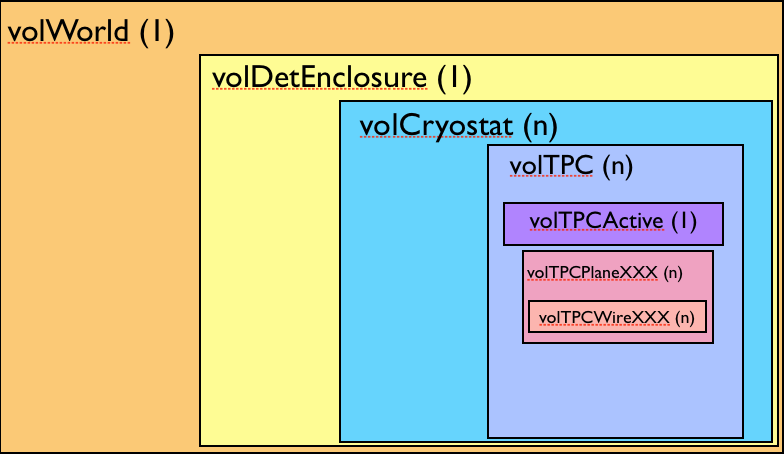
\includegraphics[width=4.0in]{./imgs/geometry_volumes.png}
\label{geo-vol.img}
\end{figure}

As shown in Figure~\ref{geo-vol.img},
the highest level volume is World which contains all elements of the geometry to be accounted for in the simulation and should be sized adequately to account for any features of the detector surroundings that are important for the simulation. For example, if there is a huge mass of rock near the detector that could alter the cosmic ray flux from that direction, it should be simulated. There is only one detector enclosure volume which can contain many Cryostat volumes, which in turn can each contain many TPC volumes. Each TPC volume contains only one TPCActive volume, which defines the active volume of liquid argon that is read out by the detector. Any liquid argon that is outside of the drift field would not be part of volTPCActive. It is assumed that volTPCActive is simply a volume of liquid argon with no sub-volumes in it. 

The TPC volume contains many TPCPlaneXXX volumes that describe the wire planes. The TPCPlaneXXX volume contains many TPCWireXXX volumes that each describe a wire in the detector. The Geant4 binding and the ROOT binding support the GDML import and export for reading GDML files and writing out GDML files.
                    
\section{Simulation Mechanics}

\subsection{Data Product Description}
LArSoft simulation jobs are modular in nature, with each module reading input data objects and writing output data objects to the event.  
As the readout electronics differ for each experiment using LArSoft, each
experiment must provide a detailed simulation of its electronics. 
\subsection{Adaptations for Using G4}
- LArSoft specific adaptations for using G4 (the user action lists and readout geometries)
The truth particles generated in the event generator step are passed to a Geant4 based detector simulation called LArG4.  The geometry GDML file is parsed to create a Geant4 detector description using the built-in GDML parser, which interfaces to LArSoft via the DetectorConstruction LArSoft class.
\subsubsection{User Action Lists}
NEED WORDS.
\subsubsection{Readout Geometries}
NEED WORDS
\subsection{Adding Additional Detectors}
- hooks for adding in additional detectors outside of the LAr volumes. 
NEED WORDS.
\subsection{New Parameterizations for Ionization}
- description of how new parameterizations for ionization, etc can be added into the simulation including a description of the mechanism for calculating the amount of ionization charge and scintillation light.  It could include a statement of the available options for that calculation (NEST vs decoupled charge and light) and how a user might add a new method.
NEED WORDS

\subsection{Incorporating Magnetic Fields}
- extensions related to incorporating magnetic fields
NEED WORDS
\subsection{Optical Simulation}
Optical physics simulations in LArSoft can take one of two forms: full or fast 
simulation.  
\subsubsection{Full Optical Simulation}
The full simulation involves stepping every optical photon individually through the detector volume.  Typical photon yields for an event cause this to be a computationally intensive procedure. The physics constructor has been specially adapted for LArSoft and includes scintillation and Cerenkov production, Rayleigh scattering, reflections at boundaries, absorption at boundaries and in the bulk, and wavelength shifting physics processes.  The configurations of these are described below.

Scintillation production is configured with a photon momentum spectrum of 9.7 ?? 1 eV and a yield of 24,000 photons per MeV of energy loss, incorporating both a fast and a slow component, which can be scaled by a quenching factor specified for each scintillating particle.  These quenching factors, and the possibility of utilizing a more systematic specification of the quenching per particle, require further investigation. Cerenkov photons are produced with yields and energies corresponding to the standard Frank-Tamm spectrum of Cerenkov radiation.\
\
Rayleigh scattering and photon-absorption process are enabled, where the scattering length is specified at 90 cm for all wavelengths and the absorption length is set to 2000 m (approximately infinite) for all wavelengths, for the purposes of preliminary studies.  The vast majority of photons produced are 128-nm scintillation photons, so we do not expect neglecting the wavelength dependence of these parameters to cause a significant problem.\
\
A simplified reflectivity model is used, whereby each type of boundary in the detector is supplied with a wavelength dependent total reflectivity and specular/diffuse reflection fraction.   For  preliminary  studies  only the  steel/argon boundaries  at  the  edge of the cryostat are  reflective,  with  all  other  surfaces,  including  wires,  field cage,  etc,  being opaque.   The steel/argon boundaries have a total reflectance of 25%, of which 50% is specular.  

\subsubsection{Fast Optical Simulation Modules}

Since the stepping of every photon generated in an event is a computationally intensive process, an alternative, fast library sampling simulation improves efficiency by not requiring stepping particles to know about the presence of optical voxels, but rather supply a modified scintillation process that fills the PhotonVoxelList with the map of scintillation photon production across the detector volume. 
The optical fiducial volume is divided into optical voxels, and the scintillation light production intensity and time profile in each voxel is recorded.  The sensitive detector configuration is somewhat different to that applied to the charge voxels, since the isotropic light production is a result of a very specific physics process.  The photon voxels are defined separately to charge voxels, since they will undergo a separate size optimization.

By comparing the intensity of the scintillation light source present in each voxel in the event to the intensity of the light sources used to generate the library file, and then applying Poisson fluctuations, a number of photons to sample for each PMT in the geometry is calculated.  A set of photons are sampled from the library file, their detection time is smeared by the time profile of scintillation in each voxel, and by combining the expected responses from the light in each voxel, a PMTHitCollection is generated representing the expected detector response for the event.

The photon library is both geometry and voxelization scheme specific, and changes to either require a full regeneration of the library, which is a one-time computationally intensive job.  The LightSource event generator supplies the intense sources of 9.7 eV photons for library generation, and all optical photons are stepped using the full optical physics simulation. The PMTHitCollections produced by LArG4 for light sources placed in each voxel, as well as the light source intensity, are stored in the library file using a module which is a part of the PhotonPropagation package.  

\section{Reconstruction Mechanics}
\subsection{Data Product Description}
The reconstruction chain proceeds in the following steps
\begin{enumerate}
\item First, the raw energy depositions (digits) are calibrated into signals on wires.
\item Next, hits are formed from the regions containing wire signals that are above a tunable threshold.
\item Hits are then grouped into clusters.
\item Clusters are classified to be projections from either 3D tracks or showers. Tracks and showers inherit from the class prong, in the usual C++ sense.
\item Vertices are located using prongs that are shown to originate from a common point.
\item Finally, prongs and vertices are associated into events.
\end{enumerate}
The LArSoft reconstruction chain is complete in that initial algorithms for each step currently exist.  More effort will be required to demonstrate that every, or at least most of the desired, event topologies can be handled in an automated way in the reconstruction chain. Detailed studies of various event classes are in progress to understand the performance of each reconstruction algorithm.

The reconstruction algorithms in LArSoft have benefited from several advances in image analysis techniques developed over the past decade.  For example, the algorithm used to cluster groups of energy depositions together is directly taken from the heavily-cited work of Ester, Kriegel, Sander, and Xu's~\cite{ester} Density Based Spatial Clustering of Applications with Noise (DBSCAN). The two-dimensional (2D) vertex, or more accurately line-endpoint, finding algorithms are based on a corner finding technique used for locating edges and corners in photographic images.  Initial particle tracking is performed using Hough line finding techniques.

\hspace*{2cm}
\begin{figure}[h]
\centering
\caption{This flow chart shows the objects created along a possible reconstruction chain in LArSoft.}
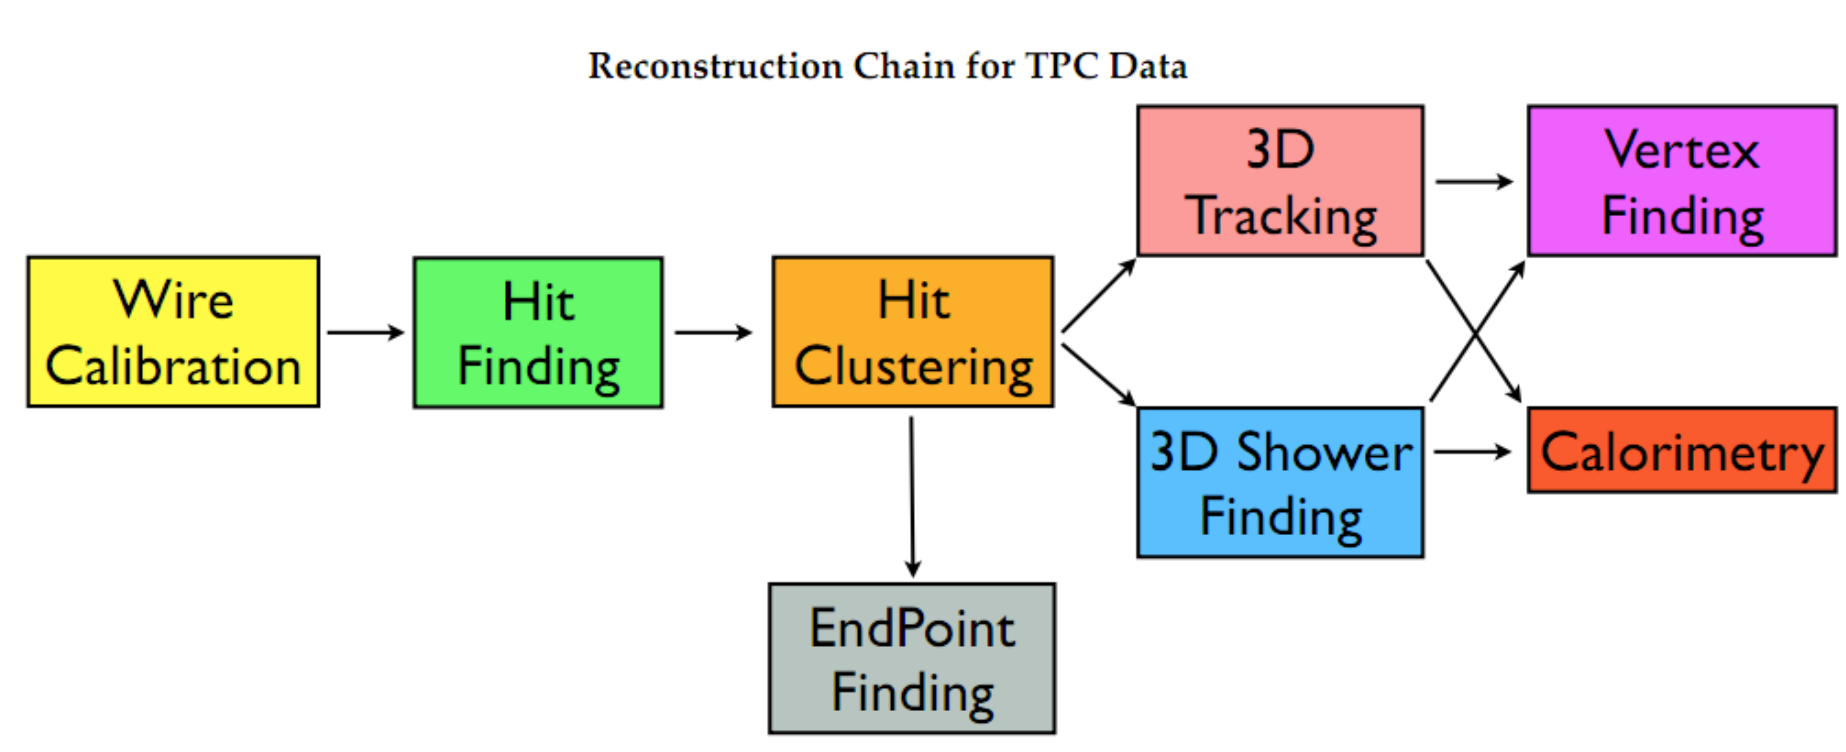
\includegraphics[width=4.0in]{./imgs/LArSoft-Recon-Flow-Soderberg.png}
\label{flow}
\end{figure}

ADD picture -- Another reconstruction chain in LArSoft

Reconstruction in LArSoft has both 2D and 3D portions. The reconstruction does not have to proceed by building 2D information before creating 3D information, but the option to do so exists. 

\subsection{Organization of Algorithms}

What is an algorithm? How do they relate to modules?

\subsection{Implementation Plan for Algorithms and Modules}
NEED WORDS.

\subsection{Unique aspects of LArSoft Reconstruction}

\subsection{Event Visualization}
LArSoft has an event display.
It can be used for
\begin{enumerate}
\item{MC}
\item{Data}
\item{2D}
\item{3D}
\end{enumerate}  

Figure~\ref{argo.evd} shows an example event display for an ArgoNeuT data event.

\hspace*{2cm}
\begin{figure}[h]
\centering
\caption{A data event in ArgoNeuT, viewed with the event display in LArSoft. Among other emitted particles, two $\pi^0$s are evident.}
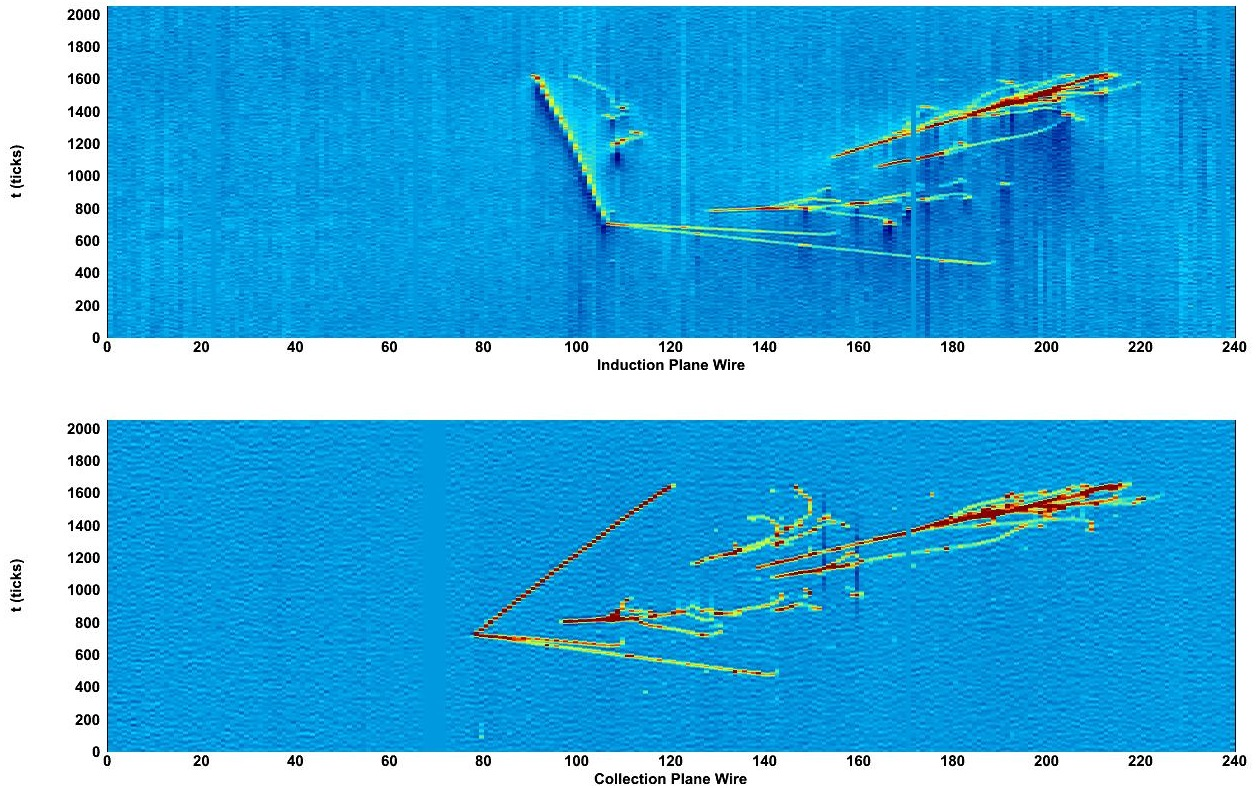
\includegraphics[width=4.0in]{./imgs/ArgoNeuT_event.jpg}
\label{argo.evd}
\end{figure}



               
\section{Analysis Mechanics}

\subsection{Data Product Description}
NEED WORDS.

\subsection{Organization of Algorithms for Analysis}
NEED WORDS.

\subsection{Implementation Plan}
NEED WORDS.

\subsection{Unique Analysis Aspects of LArSoft}
NEED WORDS.

\section{Getting Software and Benchmarking it}
\subsection{Ways to Contribute}

LArSoft is hosted in GIT repositories with ten repositories containing general software, and experiment-specific repositories for digitization code and Configuration files. MultiRepository Build (MRB) compiles code across GIT repositories. Each repository has a test area and some libraries such as EventGenerator, LArG4, HitFinder, VertexFinger, etc.\cite{gian}

Although no one has been identified to vet all code going into a release, there are spot checks and collaboration to enable everyone to be able to contribute to LArSoft. Software that is is violation of the tenants listed at \cite{code tenants} results in discussion with the appropriate experiment spokesperson. Basically, the idea is lean, modular code that is detector agnostic.  

\subsection{Unit Testing}
LArSoft does not run unit tests or regression tests, though modulo manpower has been suggested to the committee.
All LArSoft code is archived in a set of repositories based on the git version control system.
The central concepts are that no development takes place directly on the develop branch -- this is what feature branches, release branches, or hotfix branches are to be used for -- and nothing gets pushed to the reference develop branch until the changes are tested.\cite{git-control}

All LArSoft developers are expected to follow this workflow model in order to maintain the integrity of the reference "develop" and "master" branches.

Pursuant to this goal, developers are expected to fully test changes in a local branch that is up to date with the reference repository before pushing those changes to the reference develop branch. 
\subsection{Typical Memory and CPU Usage}
NEED WORDS.

\section{Summary}
NEED WORDS.
\section{References}

\begin{thebibliography}{99}
\bibitem{wcsim} https://wiki.bnl.gov/dusel/index.php/Simulation/Software
\bibitem{ester} Ester, M., Kriegel, H.-P., Sander, J., and Xu, X. 1996. "A density-based algorithm for discovering clusters in large spatial databases with noise," Proc. 2nd Int. Conf.
\bibitem{art-ref} https://cdcvs.fnal.gov/redmine/projects/artdaq
\bibitem{cry} http://nuclear.llnl.gov/simulation/
\bibitem{genie} C.Andreopoulos et al., The GENIE Neutrino Monte Carlo Generator, Nucl.Instrum.Meth.A614:87-104,2010.
\bibitem{nuwro} Tomasz Golan, Cezary Juszczak, Jan T. Sobczyk. ``Final State Interactions Effects in Neutrino-Nucleus Interaction,'' Phys.Rev. C86 (2012) 015505.
\bibitem{gibuu} O. Buss, T. Gaitanos, K. Gallmeister, H. van Hees, M. Kaskulov, O. Lalakulich, A.B. Larionov, T. Leitner, J. Weil, U. Mosel (Giessen U.). Jun 2011. ``Transport-theoretical Description of Nuclear Reactions,'' Phys.Rept. 512 (2012) 1-124. http://gibuu.hepforge.org
\bibitem{nuance} D. Casper, Nucl.Phys.Proc.Suppl. 112 (2002) 161-170
\bibitem{hepmc} Matt Dobbs (Victoria U.) , Jorgen Beck Hansen (CERN). ``The HepMC C++ Monte Carlo event record for High Energy Physics,'' Comput.Phys.Commun. 134 (2001) 41-46.
\bibitem{gian} Petrillo, Gianluca, 2014. "LArSoft: simulation and reconstruction for Liquid Argon TPC," Liquid Argon TPC R\&D Workshop, Fermilab.
\bibitem{codetenants} https://cdcvs.fnal.gov/redmine/projects/larsoft/wiki/The\_rules\_and\_guidelines
\bibitem{git-control}https://cdcvs.fnal.gov/redmine/projects/larsoft/wiki/\_The\_developer\_environment\_
\end{thebibliography}
\clearpage 

\end{document}
